\documentclass[border=4pt]{standalone}
\usepackage{mathptmx}
\usepackage[siunitx,RPvoltages]{circuitikz}
\usetikzlibrary{arrows.meta,positioning,calc}
\begin{document}
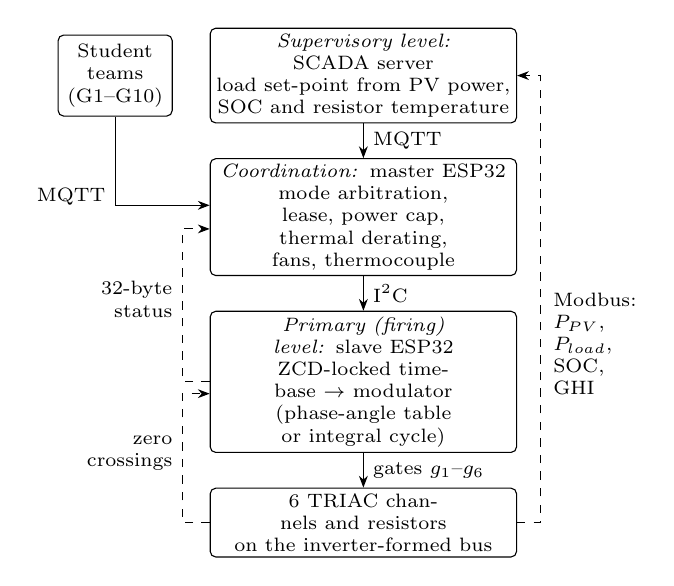
\begin{tikzpicture}[font=\scriptsize, node distance=4.4mm,
  blk/.style={draw, rounded corners=2pt, align=center, text width=3.75cm, minimum height=7mm, fill=white, inner sep=2pt},
  arr/.style={-{Stealth[length=1.5mm]}}]
\node[blk] (scada) {\textit{Supervisory level:} SCADA server\\load set-point from PV power,\\SOC and resistor temperature};
\node[blk, below=of scada] (master) {\textit{Coordination:} master ESP32\\mode arbitration, lease, power cap,\\thermal derating, fans, thermocouple};
\node[blk, below=of master] (slave) {\textit{Primary (firing) level:} slave ESP32\\ZCD-locked timebase $\rightarrow$ modulator\\(phase-angle table or integral cycle)};
\node[blk, below=of slave] (plant) {6 TRIAC channels and resistors\\on the inverter-formed bus};
\node[draw, rounded corners=2pt, align=center, fill=white, minimum height=7mm] (stud) at ([xshift=-1.2cm]scada.west |- scada) {Student\\teams\\(G1--G10)};
\draw[arr] (scada) -- node[right]{MQTT} (master);
\draw[arr] (stud.south) |- node[pos=0.45, left]{MQTT} ([yshift=1.5mm]master.west);
\draw[arr] (master) -- node[right]{I$^2$C} (slave);
\draw[arr] (slave) -- node[right]{gates $g_1$--$g_6$} (plant);
\draw[arr, dashed] (plant.east) -- ++(0.3,0) |- node[pos=0.2, right, xshift=1pt, align=left]{Modbus:\\$P_{PV}$,\\$P_{load}$,\\SOC,\\GHI} (scada.east);
\draw[arr, dashed] (slave.west) -- ++(-0.35,0) |- node[pos=0.27, left, align=right]{32-byte\\status} ([yshift=-1.5mm]master.west);
\draw[arr, dashed] (plant.west) -- ++(-0.35,0) |- node[pos=0.27, left, align=right]{zero\\crossings} ([yshift=-1.5mm]slave.west);
\end{tikzpicture}
\end{document}
